\documentclass[11pt]{article}
\usepackage[latin1]{inputenc}
\usepackage[english]{babel}
\usepackage{amsmath}
\usepackage{tikz, pgfplots}
\pgfplotsset{compat=1.9}
\raggedright
\pagestyle{empty}
\usepackage[margin = 0.5in]{geometry}
\begin{document}


Name \makebox[3in]{\hrulefill}  \hfill  Hon. PreCalc P-Set

\subsubsection*{Graphs of Other Trig Functions \hfill \makebox[0.35in]{\hrulefill} / 10}


For each of the following, state the amplitude, period, phase shift, and vertical shift. 
\begin{flalign*}
1. \quad		&	y = 1 + 3\tan(3\theta + 135^{\circ})		&
2. \quad		&	y = \sec\left(\dfrac{\theta}{4} - 135^{\circ}\right) - 1	&&\\[2in]
3. \quad		&	y = 2\csc(2\theta + 90^{\circ}) - 1	&
4. \quad		&	y = 2 + 3\cot\dfrac{\theta}{4}	&&\\[2in]
5. \quad		&	y = \dfrac{1}{2}\tan\left(2\theta - \dfrac{\pi}{2}\right) - 2	&
6. \quad		&	y = -2 + 4\sec\left(2\theta - \frac{3\pi}{4}\right)	&&\\[2in]
7. \quad		&	y = -3\tan{(2\theta + 90^{\circ})} + 1	&
8. \quad		&	y = \frac{3}{2}\sec{\theta} - 4			&&\\
\end{flalign*}



\newpage

Find the equation for each either in the form $y = a\tan{(bx)}$ or $y = a\sec{(bx)}$.
\newline\\

\begin{tabular}{p{0.5\linewidth}p{0.5\linewidth}}
9.  &   10. \\
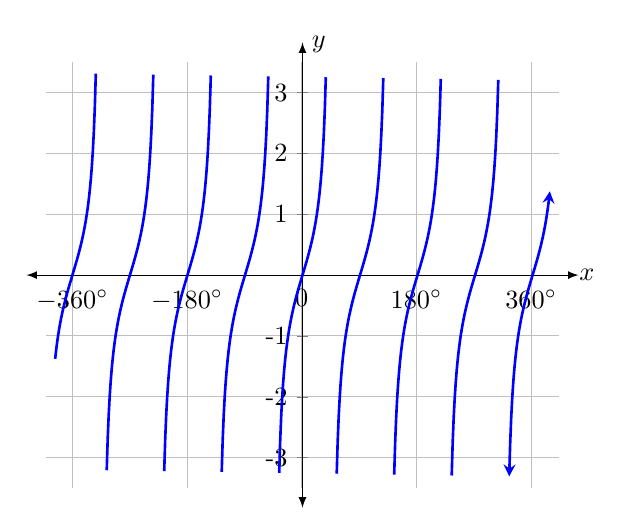
\begin{tikzpicture}[scale=0.95]

\begin{axis}
[   
    grid,
    axis lines=middle,
    xmin=-7,xmax=7,
    ymin=-3.5,ymax=3.5,
    restrict y to domain=-3.5:3.5,
    xtick={-6.28318, -3.15159265, ..., 6.28318},
    xticklabels={$-360^\circ$,$-180^\circ$,0,$180^\circ$,$360^\circ$},
    ytick={-3,-2,...,5},
    yticklabels={-3,-2,-1,,1,2,3,4,5},
    axis line style={latex-latex},
    axis line style={shorten >=-7.5pt, shorten <=-7.5pt},
    xlabel=$x$,
    ylabel=$y$,
    xlabel style={at={(ticklabel* cs:1)},anchor=west, xshift=0.15cm},
    ylabel style={at={(ticklabel* cs:1)},anchor=south west}
]
\addplot+[no marks, domain=-2.15*pi:2.15*pi, samples=500,<->, > = stealth, line width = 1]{tan(deg(2*x))};
\end{axis}

\end{tikzpicture}
&
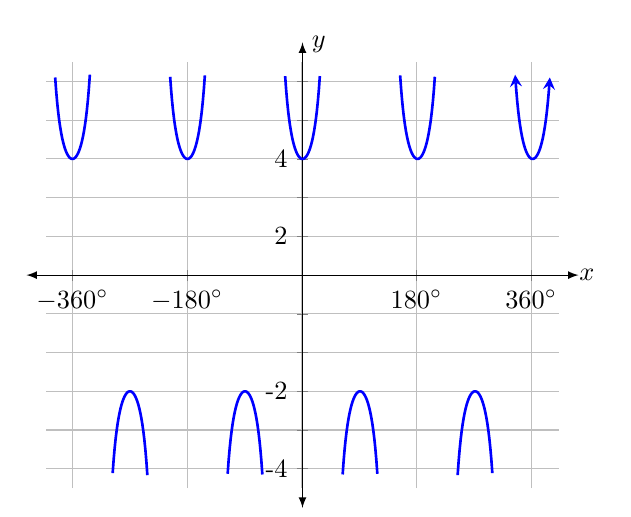
\begin{tikzpicture}[scale=0.95]

\begin{axis}
[   
    grid,
    axis lines=middle,
    xmin=-7,xmax=7,
    ymin=-5.5,ymax=5.5,
    restrict y to domain=-5.5:5.5,
    xtick={-6.28318, -3.15159265, ..., 6.28318},
    xticklabels={$-360^\circ$,$-180^\circ$,,$180^\circ$,$360^\circ$},
    ytick={-5,-4,-3,-2,...,5},
    yticklabels={-4,,-2,,,,2,,4,},
    axis line style={latex-latex},
    axis line style={shorten >=-7.5pt, shorten <=-7.5pt},
    xlabel=$x$,
    ylabel=$y$,
    xlabel style={at={(ticklabel* cs:1)},anchor=west, xshift=0.15cm},
    ylabel style={at={(ticklabel* cs:1)},anchor=south west}
]
\addplot+[no marks, domain=-2.15*pi:2.15*pi, samples=500,<->, > = stealth, line width = 1]{3*sec(deg(2*x))};
\end{axis}

\end{tikzpicture}
\end{tabular}
\bigskip


A ladder $L$ must be carried around the corner of a hallway. The hallway dimensions are shown:
\begin{center}
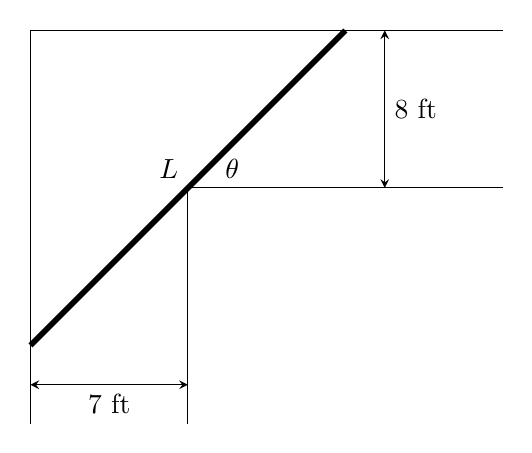
\begin{tikzpicture}
\draw (0,0) -- (6,0);
\draw (0,0) -- (0,-5);
\draw (2,-5) -- (2,-2);
\draw (2,-2) -- (6,-2);
\draw (0,-4) -- (4,0) [line width = 2];
\node at (2,-2) [anchor = south east] {$L$};
\draw [<->, > = stealth] (0,-4.5) -- (2,-4.5);
\node at (1,-4.5) [anchor = north] {7 ft};
\draw [<->, > = stealth] (4.5,0) -- (4.5,-2);
\node at (4.5,-1) [anchor = west] {8 ft};
\node at (2.35,-2) [anchor = south west] {$\theta$};
\end{tikzpicture}
\end{center}

11. Find a function $L(\theta)$ that expresses the length of the ladder in terms of $\theta$.
\\[1.5in]


12. Find the minimum value for this function.
\\[1in]


13. What is the length of the longest ladder that can be carried around this corner?
\\[1in]


14. Explain what happens to $L(\theta)$ as $\theta$ approaches 0 or $\pi/2$.



\newpage


\textbf{Graphing Other Trig Functions KEY}

\begin{enumerate}
    \item Amp = none, Per = $60^\circ$, P.S. = $45^\circ$ left, V.S. = up 1
    
    \item Amp = none, Per = $1440^\circ$, P.S. = $540^\circ$ right, V.S. = down 1
    
    \item Amp = none, Per = $180^\circ$, P.S. = $45^\circ$ left, V.S. = down 1
    
    \item Amp = none, Per = $720^\circ$, P.S. = none, V.S. = up 2
    
    \item Amp = none, Per = $\frac{\pi}{2}$, P.S. = $\frac{\pi}{4}$ right, V.S. = down 2
    
    \item Amp = none, Per = $\pi$, P.S. = $\frac{3\pi}{8}$ right, V.S. = down 2
    
    \item Amp = none, Per = $90^\circ$, P.S. = $45^\circ$ left, V.S. = up 1
    
    \item Amp = none, Per = $360^\circ$, P.S. = none, V.S. = down 4
    \end{enumerate}

\end{document}
